\documentclass[]{article}
\usepackage[a4paper, total={15cm,23cm}]{geometry}
\usepackage{fancyhdr}
\usepackage{graphicx}
\usepackage{amsmath}
\usepackage{amssymb}
\usepackage{xcolor}
\usepackage{cancel}
%opening
\title{PH 222 Activity 1}
\author{Benjamin Bauml}
\date{Winter 2021}
\pagestyle{fancy}
\rhead{PH 222}
\chead{Winter 2021}
\lhead{Activity 1}

%Custom Quotation Command
\newcommand{\excerpt}[1]{\colorbox{lightgray}{\parbox{14.8cm}{#1}} \\}

\begin{document}

\maketitle

\begin{center}
This material is borrowed/adapted from Chapter 3 of the \textit{Student Workbook} for \textit{Physics for Scientists and Engineers}, as well as from the prior term's material.
\end{center}
\section*{Activity 1}%22-24,25
\excerpt{
Write the vector in component form (e.g. $ 3\hat{\imath}+2\hat{\jmath} $).
}
\begin{center}
	\includegraphics[scale=0.9]{Ex22to24}
	%\includegraphics[scale=0.9]{Ex22to24Sol}%Solution
\end{center}
\excerpt{
What is the vector sum $ \vec{D} = \vec{A} + \vec{B} + \vec{C} $ of the three aforementioned vectors? Write your answer in component form.
}
% To reveal the solution, delete "\phantom{\parbox{\textwidth}{" from the beginning, and "}}" from the end.
\phantom{\parbox{\textwidth}{
\[
\vec{D} = (3-1-3)\hat{\imath} + (1-2+0)\hat{\jmath} = -\hat{\imath}-\hat{\jmath}
\]
}}

\section*{Activity 2}%29-31
\excerpt{
Define vector $ \vec{A} = (5,\ 30^{\circ}\text{ above the horizontal}) $. Determine the components $ A_{x} $ and $ A_{y} $ in the three coordinate systems shown below. Show your work below the figure.
}
\begin{center}
	\includegraphics[scale=0.9]{Ex29to31}
	%\includegraphics[scale=0.9]{Ex29to31Sol}%Solution
\end{center}

\pagebreak
\section*{Activity 3}%Quiz 8 reframed
\excerpt{
The Fabulous Topperweins, Elizabeth and her husband Ad, are attempting a truly daring trick shot. Ad fires his shotgun due east, with the slug having speed $ v_{0s} $ and mass $ m_{s} $. Simultaneously, Elizabeth fires her pistol from the northeast, at an angle $ \phi $ south of west. Her bullet (with mass $ m_{b} $) strikes Ad's slug with speed $ v_{0b} $. The impact releases enough heat to melt the two projectiles together. After the collision, the bullet and slug fly as one body at some unknown velocity. Find the final speed and direction angle of the two projectiles after the collision.
}
\begin{center}
	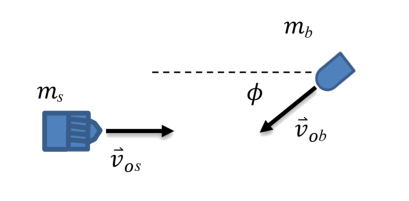
\includegraphics[scale=1.2]{OverBroadway}
\end{center}
\excerpt{
(A) Establish a coordinate system and clearly label the axes. Use this coordinate system to draw before and after pictures of the collision, clearly showing/labeling vectors and angles. Write down what is given (known) from the problem statement and what you want to find (unknowns).
}
% To reveal the solution, delete "\phantom{\parbox{\textwidth}{" from the beginning, and "}}" from the end.
\phantom{\parbox{\textwidth}{
\begin{center}
	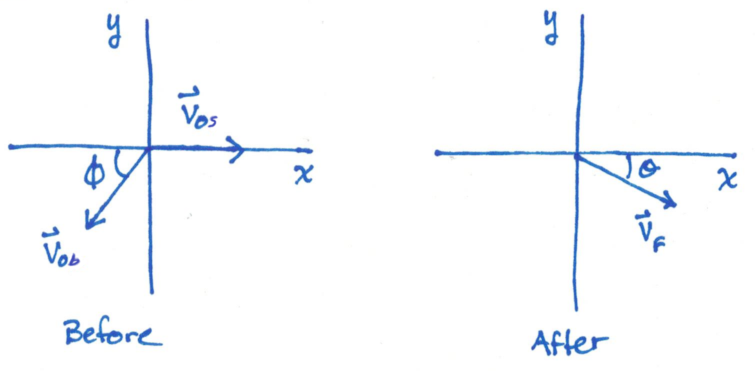
\includegraphics{Representations}
\end{center}
Known: $ m_{s},\ m_{b},\ v_{0s},\ v_{0b},\ \phi $ \\
Unknown: $ v_{f} = \sqrt{v_{fx}^{2}+v_{fy}^{2}},\ \theta = \arctan(v_{fy}/v_{fx}) $ \\
}}
\excerpt{
(B) Write down the conservation of momentum equation(s) in symbolic form for the collision using your coordinate system from part (A). Do not solve or simplify.
}
% To reveal the solution, delete "\phantom{\parbox{\textwidth}{" from the beginning, and "}}" from the end.
\phantom{\parbox{\textwidth}{
When momentum is conserved, we know that the sum of all initial momenta is equal to the sum of all final momenta. In this particular case, that means
\[
m_{s}\vec{v}_{0s} + m_{b}\vec{v}_{0b} = (m_{s}+m_{b})\vec{v}_{f}.
\]
Breaking this expression into components, we obtain
\[
\begin{split}
	m_{s}v_{0s} - m_{b}v_{0b}\cos\phi & = (m_{s}+m_{b})v_{fx}; \\
	- m_{b}v_{0b}\sin\phi & = (m_{s}+m_{b})v_{fy}.
\end{split}
\]
}}
\excerpt{
(C) Suppose that $ v_{0s} = 500 $ m/s, $ m_{s} = 0.025 $ kg, $ v_{0b} = 600 $ m/s, $ m_{b} = 0.01 $ kg, and $ \phi = 30^{\circ} $. Determine the final speed of the two projectiles after the collision. Check units.
}
% To reveal the solution, delete "\phantom{\parbox{\textwidth}{" from the beginning, and "}}" from the end.
\phantom{\parbox{\textwidth}{
\[
\begin{split}
	v_{f} & = \sqrt{v_{fx}^{2}+v_{fy}^{2}} \\
	& = \sqrt{\left(\frac{m_{s}v_{0s} - m_{b}v_{0b}\cos\phi}{m_{s}+m_{b}}\right)^{2}+\left(\frac{- m_{b}v_{0b}\sin\phi}{m_{s}+m_{b}}\right)^{2}} \\
	& = \frac{1}{m_{s}+m_{b}} \sqrt{m_{s}^{2}v_{0s}^{2} - 2m_{s}m_{b}v_{0s}v_{0b}\cos\phi + m_{b}^{2}v_{0b}^{2}\cos^{2}\phi + m_{b}^{2}v_{0b}^{2}\sin^{2}\phi} \\
	& = \frac{1}{m_{s}+m_{b}} \sqrt{m_{s}^{2}v_{0s}^{2} - 2m_{s}m_{b}v_{0s}v_{0b}\cos\phi + m_{b}^{2}v_{0b}^{2}} \\
	& \approx \frac{1}{0.035\text{ kg}} \sqrt{156.25\text{ kg}^{2}\text{m}^{2}\text{/s}^{2} - 129.9\text{ kg}^{2}\text{m}^{2}\text{/s}^{2} + 36\text{ kg}^{2}\text{m}^{2}\text{/s}^{2}} \\
	& = \frac{1}{0.035\text{ kg}} \sqrt{62.35\text{ kg}^{2}\text{m}^{2}\text{/s}^{2}} \\
	& \approx 225 \text{ m/s}
\end{split}
\]
}}
\excerpt{
(D) Suppose that $ v_{0s} = 500 $ m/s, $ m_{s} = 0.025 $ kg, $ v_{0b} = 600 $ m/s, $ m_{b} = 0.01 $ kg, and $ \phi = 30^{\circ} $. Determine the direction angle of the two projectiles after the collision. Check units.
}
% To reveal the solution, delete "\phantom{\parbox{\textwidth}{" from the beginning, and "}}" from the end.
\phantom{\parbox{\textwidth}{
\[
\begin{split}
	\theta & = \arctan\left(\frac{v_{fy}}{v_{fx}}\right) \\
	& = \arctan\left(\frac{- m_{b}v_{0b}\sin\phi}{m_{s}v_{0s} - m_{b}v_{0b}\cos\phi}\right) \\
	& = \arctan\left(\frac{- (6\text{ kg m/s})\sin(30^{\circ})}{12.5\text{ kg m/s} - (6\text{ kg m/s})\cos(30^{\circ})}\right) \\
	& \approx \arctan\left(\frac{- 3\text{ kg m/s}}{7.3\text{ kg m/s}}\right) \\
	& \approx -22.3^{\circ}
\end{split}
\]
It is important to check whether or not this angle makes sense. Since $ v_{fx} $ is positive and $ v_{fy} $ is negative, we know that our vector should be in the fourth quadrant. Pointing 22.3 degrees below the horizontal is consistent with our expectations.
}}

\end{document}